%!TEX root = ../Thesis.tex

\section{Skip-gram}

The Skip-gram model tries to learn the meaning of words by its context. Specifically it tries to predict the surrounding words given a single input word.

The Skip-gram model does this by by encoding the input word using 1-of-V encoding where $V$ is the vocabulary size. This means that each word is represented as an indicator vector, where the indicator represent a single word from a given vocabulary. The vocabulary is typically defined using the $V$ most common word in the text corpus. \marginnote{\vspace{-1.5cm}\textbf{corpus}: \\ collection of documents}
\begin{figure}[h]
\begin{equation*}
\begin{aligned}
\text{twinkle}: \left[1, 0, 0, 0, \cdots \right] \\
\text{twinkle}: \left[1, 0, 0, 0, \cdots \right] \\
\text{little}: \left[0, 1, 0, 0, \cdots \right] \\
\text{star}: \left[0, 0, 1, 0, \cdots \right]
\end{aligned}
\end{equation*}
\caption{Example of 1-of-V encoding on the sentense ``twinkle twinkle little star''}
\end{figure}

Each of these word representations are then transformed intro a lower dimensional space (latent representation). In this space words with same meaning should be close to each other. The position of each word should also contain a higher semantic meaning, such that for example $f(King) - f(Man) + f(Female) \approx f(Queen)$ \cite{word2vec-comparing}. Here $f$ is the transformation function from the input space to the latent representation.

The model is trained such that the surrounding words can be predicted from this latent representation. See Figure \ref{fig:theory:skip-gram:graph} for a graphical overview. An important detail about this model, is that the order of the words within the considered text window have no effect on the training. Thus all surrounding are assumed to having approximatly the same meaning.

\begin{figure}[h]
	\centering
	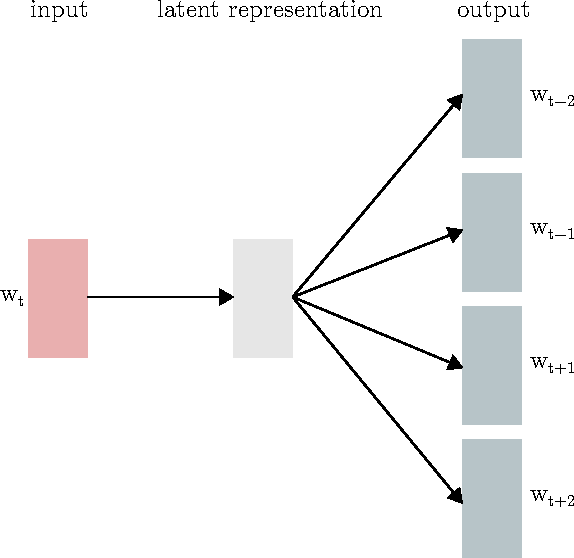
\includegraphics[scale=0.7]{theory/skip-gram-graph}
	\caption{Visualization of the Skip-gram model. Given a single input word it tries to predict the surrounding words. From this the latent representation is learned.}
	\label{fig:theory:skip-gram:graph}
\end{figure}

\subsection{The likelihood function}
The Skip-gram model is optimized by maximum-likelihood. Given a corpus with $\mathcal{D}$ documents where each document have $T_d$ words, the likelihood function is calculated using the conditional probability of observing the surrounding words ($w_{d, t + \ell}$) given the input words ($w_{d, t}\. , t \in [1, T_d]$).
\begin{equation}
\prod_{d = 1}^{\mathcal{D}} \prod_{t = 1}^{T_d} \prod_{\ell} p(w_{d, t + \ell} | w_{d, t})
\label{eq:theory:skipgram:full-likelihood}
\end{equation}

The details about which document there currently is used, are typically omitted from the expressions. Thus equation \eqref{eq:theory:skipgram:full-likelihood} becomes:
\begin{equation}
\prod_{t = 1}^{T} \prod_{\ell} p(w_{t + \ell} | w_{t})
\end{equation}

Since words closer to $w_t$ are expected to be more related to that word, the near surrounding words are weighed higher. This is not modelled by explicit weights, but instead by letting $\ell \in [-R, R] \setminus \{ 0 \}$ where $R \sim U[1, C]$ \cite{word2vec-comparing}.

For easier optimization of the likelihood function, the average log likelihood is used instead \todo{Consider a minus sign here for consistency}:
\begin{equation}
\mathcal{L} = \frac{1}{T} \sum_{t = 1}^T \sum_{\ell} \ln( p(w_{t + \ell} | w_t) )
\end{equation}

\subsection{Forward pass}
The conditional probability $p(w_{t + \ell} | w_t)$ is calculated using a log-linear model. This is best explained by considering a neural network, with a single hidden layer and no non-linear units ($\theta(a) = a$).

\begin{figure}[H]
	\centering
	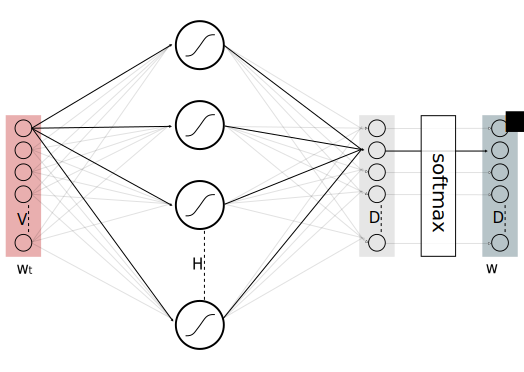
\includegraphics[scale=0.7]{theory/skip-gram-network}
	\caption{Visualization of a single pass though the Skip-gram network.}
\end{figure}

To get an idea about how a neural network representation relates to the equations in \cite{word2vec-details}, the scalar notation from the introduction to Neural Network section is replaced with a similar vector notation.

As previously discussed the input and output words are represented using 1-of-V encoding, this vector will be denoted as $\mathbf{x}_w$ for both the input and output words $w$. Note that because words are used as input, there is a finite amount of possible inputs. The activation is thus not denoted by the input index $n$ but rather the input value $w$. For referring to the word at position $t$ in the corpus $w_t$ is used.

The activation in the hidden layer is:
\begin{equation}
\mathbf{b}_{1,w} = \mathbf{a}_{1,w} = \mathbf{W}_{1} \mathbf{x}_w
\end{equation}

Here the subscript $1$ denotes that this is for the layer 1 (the input is layer 0). The output before the softmax is applied is then calculated as:
\begin{equation}
\mathbf{a}_{2,w} = \mathbf{W}_2^T \mathbf{b}_{1,w}
\end{equation}

Here $\mathbf{W}_1$ is the matrix containing the weights on the left side of the log-linear network, thus it has a size of $D \times V$. $\mathbf{W}_2$ is the matrix containing the weights on the right side and have also size $D \times V$.

$\mathbf{a}_{2,w}$ is a vector containing information about all possible surrounding words, but since this used in a softmax and likelihood setting, only the value associated with the output word $w_{t + \ell}$ is of interrest. To get this specific value the encoding vector $\mathbf{x}_{t + \ell}$ can be used. In general the value associated with the word $k$ can be obtained using:
\begin{equation}
a_{w,k} = \left(\mathbf{a}_{2,w}\right)_k = \mathbf{x}_{k}^T \mathbf{a}_{2,w}
\end{equation}
This detail is not particular important, but explains the some of the notation used in \cite{word2vec-details}.

The probability $p(w_{t + \ell} | w_t)$ can now be calculated using a softmax:
\begin{equation}
\begin{aligned}
p(w_{t + \ell} | w_t)
&= \frac{\exp(a_{w_t,k})}{\sum_{k'=1}^K \exp(a_{w_t,k'})}
= \frac{\exp(a_{w_t, w_{t + \ell}})}{\sum_{w=1}^V \exp(a_{w_t, w})} \\
&= \frac{\exp( \mathbf{x}_{w_{t+\ell}}^T \mathbf{a}_{2,w_t} )}{\sum_{w=1}^V \exp(\mathbf{x}_{w}^T \mathbf{a}_{2,w_t})}
= \frac{
	\exp( \mathbf{x}_{w_{t+\ell}}^T \mathbf{W}_2^T \mathbf{W}_1 \mathbf{x}_{w_{t+\ell}})
}{
	\sum_{w=1}^V \exp(\mathbf{x}_{w}^T \mathbf{W}_2^T \mathbf{W}_1 \mathbf{x}_{w_{t+\ell}})
} \\
&= \frac{
	\exp( \left(\mathbf{W}_2 \mathbf{x}_{w_{t+\ell}} \right)^T \mathbf{W}_1 \mathbf{x}_{w_{t+\ell}})
}{
	\sum_{w=1}^V \exp( \left(\mathbf{W}_2 \mathbf{x}_{w}\right)^T \mathbf{W}_1 \mathbf{x}_{w_{t+\ell}})
}
\end{aligned}
\end{equation}

From the above expression it's seen that $a_{w_t, w_{t + \ell}}$ is really an inner product between two linear vector transformations. This is similar to how \cite{word2vec-details} represents the model. Specifically it one sets: $w_O = w_{t + \ell}$, $w_I = w_t$, $\mathbf{v}_{w_O} = \mathbf{W}_2 \mathbf{x}_{w_{t+\ell}}$, $\mathbf{v}_{w} = \mathbf{W}_2 \mathbf{x}_{w}$ and $\mathbf{v}_{w_I} = \mathbf{W}_1 \mathbf{x}_{w_{t + \ell}}$, then \cite[eq. 2]{word2vec-details} is obtained:
\begin{equation}
p(w_O | w_I) = \frac{
	\mathrm{exp}( \mathbf{v}_{w_O}^T \mathbf{v}_{w_I} )
}{
	\sum_{w=1}^V \mathrm{exp}( \mathbf{v}_{w}^T \mathbf{v}_{w_I} )
}
\end{equation}

This calculation is problematic since it involves a sum over all words in the vocabulary. In the Skip-gram model the vocabulary can be of size $10^5$ to $10^7$ \cite{word2vec-details}. This is why \cite{word2vec-comparing, word2vec-details, word2vec-explained} uses an approximation in form of either \textit{hierarchical softmax} or \textit{negative-sampling}. These approximations will not be discussed here, but are worth considering as they will reduce the computational complexity from $\mathcal{O}(V)$ to $\mathcal{O}(\ln_2(V))$ \cite{word2vec-comparing}.

\subsection{Backward pass}

\todo[inline]{Rewrite this to use the new notation and backpropergation. Should it stay in vector notation. It might be confusing since no other part of this report uses the vector notation.}

Since there is no closed-form solution to this maximum-likelihood problem, gradient descent is used to iteratively optimize the parameters $\mathbf{W}_O$ and $\mathbf{W}_I$. This is done by deriving the derivatives for the average log likelihood function. 
\begin{equation}
\frac{\partial}{\partial \mathbf{W}} \frac{1}{T} \ln( \mathcal{L} ) = \frac{1}{T} \sum_{t = 1}^T \sum_{\ell} \frac{\partial}{\partial \mathbf{W}} \ln( p(w_{t + \ell} | w_t) )
\end{equation}
Here $\mathbf{W}$ symbolizes both the parameters in $\mathbf{W}_O$ and in $\mathbf{W}_I$. 
\begin{equation*}
\centerline{$
\begin{aligned}
\frac{\partial}{\partial \mathbf{W}} \ln( p(w_O | w_I) ) &= \frac{\partial}{\partial \mathbf{W}} 	 \left( \frac{
	\mathrm{exp}( \left( \mathbf{W}_O \mathbf{x}_{w_O} \right)^T \mathbf{W}_I \mathbf{x}_{w_I} )
}{
	\sum_{w=1}^V \mathrm{exp}( \left( \mathbf{W}_O \mathbf{x}_{w} \right)^T \mathbf{W}_I \mathbf{x}_{w_I} )
} \right) \\
&= \frac{\partial}{\partial \mathbf{W}} \left( \left( \mathbf{W}_O \mathbf{x}_{w_O} \right)^T \mathbf{W}_I \mathbf{x}_{w_I} - \ln \left(\sum_{w=1}^V \mathrm{exp}( \left( \mathbf{W}_O \mathbf{x}_{w} \right)^T \mathbf{W}_I \mathbf{x}_{w_I}) \right) \right) \\
&= \frac{\partial}{\partial \mathbf{W}} \left( \mathbf{W}_O \mathbf{x}_{w_O} \right)^T \mathbf{W}_I \mathbf{x}_{w_I} - \frac{
	\frac{\partial}{\partial \mathbf{W}} \sum_{w=1}^V \mathrm{exp}( \left( \mathbf{W}_O \mathbf{x}_{w} \right)^T \mathbf{W}_I \mathbf{x}_{w_I})
} {
	\sum_{w=1}^V \mathrm{exp}( \left( \mathbf{W}_O \mathbf{x}_{w} \right)^T \mathbf{W}_I \mathbf{x}_{w_I})
} \\
&= \frac{\partial}{\partial \mathbf{W}} \left( \mathbf{W}_O \mathbf{x}_{w_O} \right)^T \mathbf{W}_I \mathbf{x}_{w_I} - \frac{
	\sum_{w=1}^V \left(\frac{\partial}{\partial \mathbf{W}} \left(\mathbf{W}_O \mathbf{x}_{w} \right)^T \mathbf{W}_I \mathbf{x}_{w_I} \right) \mathrm{exp}( \left( \mathbf{W}_O \mathbf{x}_{w} \right)^T \mathbf{W}_I \mathbf{x}_{w_I})
} {
	\sum_{w=1}^V \mathrm{exp}( \left( \mathbf{W}_O \mathbf{x}_{w} \right)^T \mathbf{W}_I \mathbf{x}_{w_I})
}
\end{aligned}$}
\end{equation*}

At this point it becomes necessary to distinguish between the elements in $\mathbf{W}_O$ and $\mathbf{W}_I$.

\begin{equationbox}[H]
\begin{equation*}
\begin{aligned}
\frac{\partial}{\partial \mathbf{W}_I} \ln( p(w_O | w_I) ) = \mathbf{W}_O \mathbf{x}_{w_O} \mathbf{x}_{w_I}^T - \frac{
	\sum_{w=1}^V \mathbf{W}_O \mathbf{x}_{w} \mathbf{x}_{w_I}^T \mathrm{exp}( \left( \mathbf{W}_O \mathbf{x}_{w} \right)^T \mathbf{W}_I \mathbf{x}_{w_I})
} {
	\sum_{w=1}^V \mathrm{exp}( \left( \mathbf{W}_O \mathbf{x}_{w} \right)^T \mathbf{W}_I \mathbf{x}_{w_I})
} \\
\frac{\partial}{\partial \mathbf{W}_O} \ln( p(w_O | w_I) ) = \mathbf{W}_I \mathbf{x}_{w_I} \mathbf{x}_{w_O}^T - \frac{
	\sum_{w=1}^V \mathbf{W}_I \mathbf{x}_{w_I} \mathbf{x}_{w}^T \mathrm{exp}( \left( \mathbf{W}_O \mathbf{x}_{w} \right)^T \mathbf{W}_I \mathbf{x}_{w_I})
} {
	\sum_{w=1}^V \mathrm{exp}( \left( \mathbf{W}_O \mathbf{x}_{w} \right)^T \mathbf{W}_I \mathbf{x}_{w_I})
}
\end{aligned}
\end{equation*}
\caption{Derivatives for the Skip-Gram model}
\end{equationbox}
\marginnote{\vspace{-3cm}Remember \cite{matrix-cookbook}:\\  ${\frac{\partial \mathbf{a}^T X \mathbf{b}}{\partial X} = \mathbf{a} \mathbf{b}^T}$, ${\frac{\partial \mathbf{a}^T X^T \mathbf{b}}{\partial X} = \mathbf{b} \mathbf{a}^T}$}

